\documentclass[a4paper]{article}
\usepackage{times}
\usepackage[utf8]{inputenc}
\usepackage{selinput}
\usepackage{upquote}
\usepackage[margin=2cm, rmargin=4cm, tmargin=3cm]{geometry}
\usepackage{tcolorbox}
\usepackage{xspace}
\usepackage[french]{babel}
\usepackage{url}
\usepackage{hyperref}
\usepackage{fontawesome5}
\usepackage{marginnote}
\usepackage{ulem}
\usepackage{tcolorbox}
\usepackage{graphicx}
%\usepackage[top=Bcm, bottom=Hcm, outer=Ccm, inner=Acm, heightrounded, marginparwidth=Ecm, marginparsep=Dcm]{geometry}


\newtcolorbox{Example}[1]{colback=white,left=20pt,colframe=slideblue,fonttitle=\bfseries,title=#1}
\newtcolorbox{Solutions}[1]{colback=white,left=20pt,colframe=green,fonttitle=\bfseries,title=#1}
\newtcolorbox{Conseils}[1]{colback=white,left=20pt,colframe=slideblue,fonttitle=\bfseries,title=#1}
\newtcolorbox{Warning}[1]{colback=white,left=20pt,colframe=warning,fonttitle=\bfseries,title=#1}

\setlength\parindent{0pt}

  %Exercice environment
  \newcounter{exercice}
  \newenvironment{Exercice}[1][]
  {
  \par
  \stepcounter{exercice}\textbf{Question \arabic{exercice}:} (\faClock \enskip \textit{#1})
  }
  {\bigskip}
  

% Title
\newcommand{\titre}{\begin{center}
  \section*{Algorithmes et Pensée Computationnelle}
\end{center}}
\newcommand{\cours}[1]
{\begin{center} 
  \textit{#1}\\
\end{center}
  }


\newcommand{\exemple}[1]{\newline~\textbf{Exemple :} #1}
%\newcommand{\attention}[1]{\newline\faExclamationTriangle~\textbf{Attention :} #1}

% Documentation url (escape \# in the TP document)
\newcommand{\documentation}[1]{\faBookOpen~Documentation : \href{#1}{#1}}

% Clef API
\newcommand{\apikey}[1]{\faKey~Clé API : \lstinline{#1}}
\newcommand{\apiendpoint}[1]{\faGlobe~Url de base de l'API \href{#1}{#1}}

%Listing Python style
\usepackage{color}
\definecolor{slideblue}{RGB}{33,131,189}
\definecolor{green}{RGB}{0,190,100}
\definecolor{blue}{RGB}{121,142,213}
\definecolor{grey}{RGB}{120,120,120}
\definecolor{warning}{RGB}{235,186,1}

\usepackage{listings}
\lstdefinelanguage{texte}{
    keywordstyle=\color{black},
    numbers=none,
    frame=none,
    literate=
           {é}{{\'e}}1
           {è}{{\`e}}1
           {ê}{{\^e}}1
           {à}{{\`a}}1
           {â}{{\^a}}1
           {ù}{{\`u}}1
           {ü}{{\"u}}1
           {î}{{\^i}}1
           {ï}{{\"i}}1
           {ë}{{\"e}}1
           {Ç}{{\,C}}1
           {ç}{{\,c}}1,
    columns=fullflexible,keepspaces,
	breaklines=true,
	breakatwhitespace=true,
}
\lstset{
    language=Python,
	basicstyle=\bfseries\footnotesize,
	breaklines=true,
	breakatwhitespace=true,
	commentstyle=\color{grey},
	stringstyle=\color{slideblue},
  keywordstyle=\color{slideblue},
	morekeywords={with, as, True, False, Float, join, None, main, argparse, self, sort, __eq__, __add__, __ne__, __radd__, __del__, __ge__, __gt__, split, os, endswith, is_file, scandir, @classmethod},
	deletekeywords={id},
	showspaces=false,
	showstringspaces=false,
	columns=fullflexible,keepspaces,
	literate=
           {é}{{\'e}}1
           {è}{{\`e}}1
           {ê}{{\^e}}1
           {à}{{\`a}}1
           {â}{{\^a}}1
           {ù}{{\`u}}1
           {ü}{{\"u}}1
           {î}{{\^i}}1
           {ï}{{\"i}}1
           {ë}{{\"e}}1
           {Ç}{{\,C}}1
           {ç}{{\,c}}1,
    numbers=left,
}

\newtcbox{\mybox}{nobeforeafter,colframe=white,colback=slideblue,boxrule=0.5pt,arc=1.5pt, boxsep=0pt,left=2pt,right=2pt,top=2pt,bottom=2pt,tcbox raise base}
\newcommand{\projet}{\mybox{\textcolor{white}{\small projet}}\xspace}
\newcommand{\optionnel}{\mybox{\textcolor{white}{\small Optionnel}}\xspace}
\newcommand{\advanced}{\mybox{\textcolor{white}{\small Pour aller plus loin}}\xspace}
\newcommand{\auto}{\mybox{\textcolor{white}{\small Auto-évaluation}}\xspace}


\usepackage{environ}
\newif\ifShowSolution
\NewEnviron{solution}{
  \ifShowSolution
	\begin{Solutions}{\faTerminal \enskip Solution}
		\BODY
	\end{Solutions}
  \fi}


  \usepackage{environ}
  \newif\ifShowConseil
  \NewEnviron{conseil}{
    \ifShowConseil
    \begin{Conseils}{\faLightbulb \quad Conseil}
      \BODY
    \end{Conseils}

    \fi}

    \usepackage{environ}
  \newif\ifShowWarning
  \NewEnviron{attention}{
    \ifShowWarning
    \begin{Warning}{\faExclamationTriangle \quad Attention}
      \BODY
    \end{Warning}

    \fi}
  

%\newcommand{\Conseil}[1]{\ifShowIndice\ \newline\faLightbulb[regular]~#1\fi}


\usepackage{array}
\newcolumntype{C}[1]{>{\centering\let\newline\\\arraybackslash\hspace{0pt}}m{#1}}

\begin{document}
% Change the following values to true to show the solutions or/and the hints
\ShowSolutiontrue
\ShowConseiltrue
\titre
\cours{Programmation orientée objet}
% TODO: Objectifs à atteindre (Alpha)

% TODO (All): Utiliser \lstinline{} sur tous les mots-clés, noms de classes, d'attributs, méthodes,...

% TODO (All): À aucun moment on ne parle de constructeur par défaut! Il s'agit d'une notion importante en POO que nous devons aborder.
Le code présenté dans les énoncés se trouve sur Moodle, dans le dossier \lstinline{Ressources}.

\section{Création de votre première classe en Java}

Le but de cette première partie est de créer votre propre classe en Java. Cette classe sera une classe nommée Dog() sensée représenter un chien.

Cette classe aura différents attributs et différentes ,méthodes que vous implémenterez au fur et à mesure de l'exercice. 

\begin{Exercice}[10 minutes] Exercice 1\\
    Commencez par créer une nouvelle Java Class dans votre projet, et initialisez les attributs suivants :
    \begin{enumerate}
    \item Un attribut public String nommé \lstinline{name}
    \item Un attribut privé List nommé tricks
    \item Un attribut privé String nommé race
    \item Un attribut privé int nommé age
    \item Un attribut privé int nommé mood initialisé à 5(correspondant à l'humeur du chien)
    \item Un attribut privé de classe (static) int nommé nb\_chiens
   	\end{enumerate}
   	
   	Ensuite, créez une méthode publique du même nom que la classe (Dog), qui va servir à initialiser nos différentes instances de cette classe. Cette méthode prendra en argument les éléments suivants et initialisera les attributs de notre instance avec :
   	\begin{enumerate}
    \item Une chaîne de caractère \lstinline{name}
    \item Une liste tricks
    \item Une chaîne de caractère race
    \item Un entier age
   	\end{enumerate}
   	
   	Pour finir, cette méthode doit incrémenter l'attribut de classe nb\_chiens qui va garder en mémoire le nombre d'instances crées.
   	
\begin{conseil}
   N'oubliez pas de préciser si vos attributs sont \lstinline{public} ou \lstinline{private}.
   
   Le mot \lstinline{static} correspond à un élément de classe (attribut ou méthode), cet élément pourra ensuite être appelé via la classe directement.
\end{conseil}
    
\begin{solution}
	\lstinputlisting{ressources/Question1.java}
\end{solution}
\end{Exercice}

\begin{Exercice}[10 minutes] Exercice 2\\
    Il faut maintenant créer des méthodes nommées setter et getter pour les attributs privés. Ce sont ces méthodes qui vous permettront d'interagir avec les attributs privés de la fonction. Pour les attributs publics, il vous suffit d'utiliser nom\_instance.attribut pour l'obtenir. \\
    
    Les méthodes getter consistent à retourner la valeur de l'attribut. Les setter consisteront à modifier la valeur de l'attribut. Les \lstinline{setter} sont souvent utilisés pour modifier la valeur d'attributs privés. \\
    
    Créez les méthodes suivantes :
    \begin{enumerate}
    \item getTricks()
    \item getRace()
    \item getAge()
    \item getMood()
    \item setTricks()
    \item setRace()
    \item setAge()
    \item setMood()
    \end{enumerate}
    
    Créez également une méthode de classe permettant de retourner le nombre de chiens instanciés (une méthode getter).
   	
\begin{conseil}
   Les setter et getter vous seront proposés via l'autocompletion d'Intellij, nous vous recommandons tout de même d'en faire quelques unes à la main.
\end{conseil}
    
\begin{solution}
	\lstinputlisting{ressources/Question2.java}
\end{solution}
\end{Exercice}

\begin{Exercice}[5 minutes] Exercice 3\\
    Créez une méthode nommée \lstinline{add_trick} qui prend en entrée une chaîne de caractère et l'ajoute à la liste \lstinline{tricks}. \\
   	
\begin{conseil}
   La liste \lstinline{tricks} est une liste comme les autres. Si vous voulez la modifier, vous aurez besoin de passer par une LinkedList temporaire.
\end{conseil}
    
\begin{solution}
	\lstinputlisting{ressources/Question3.java}
\end{solution}
\end{Exercice}

\begin{Exercice}[5 minutes] Exercice 4\\
    Créez deux méthodes qui vont avoir un impact sur l'attribut mood du chien. La méthode leash() décrémentera mood de 3 et eat() l'incrémentera de 2. \\

\begin{solution}
	\lstinputlisting{ressources/Question4.java}
\end{solution}
\end{Exercice}

\begin{Exercice}[5 minutes] Exercice 5\\
    Créez une méthode nommée get\_oldest qui prend en argument un élément de type Dog, puis retourne le nom et l'age du chien le plus agé sous le format suivant : "nom\_chien est le chien le plus agé avec age\_chien ans". \\
   	
\begin{conseil}
   L'élément Dog que vous passez en argument est un objet de type Dog, vous pouvez donc lui appliquer les méthodes que vous avez créé tout à l'heure.
   Faites attention à la façoon d'accéder aux différents attributs de votre deuxième chien (public vs private).
\end{conseil}
    
\begin{solution}
	\lstinputlisting{ressources/Question5.java}
\end{solution}
\end{Exercice}

\begin{Exercice}[5 minutes] Exercice 6\\
    Créez une méthode de surcharge de la fonction System.out.println pour les objets de type Dog. Pour ce faire, le nom de votre méthode doit être le suivant : toString(). \\
    Veillez à retourner une chaîne de caractère sous le format suivant : nom\_chien a age\_chien ans, est un race\_chien et a une humeur de mood\_chien. Il sait faire les tours suivants : tricks\_chien.

    % TODO: Donner plus de détails sur le rôle de la méthode toString() et expliquer le but de la surcharge. Dans ce cas, toString est héritée de la super classe Object. Etant donné qu'ils n'ont pas fait de POO, autant mieux utiliser un autre exemple de surcharge de méthode ou trouver un moyen de leur dire qu'ils verront plus en détails lorsqu'on fera l'héritage.

\begin{solution}
	\lstinputlisting{ressources/Question6.java}
\end{solution}
\end{Exercice}

Pour contrôler que vos méthodes et attributs ont été implémentés correctement, vous pouvez essayer le code suivant dans votre classe Main :

	\lstinputlisting{ressources/maingaetan.java}
	
Vous devriez obtenir ce résultat :

    \lstinputlisting{ressources/mainsolution.java}
% TODO: Dans cet exercice, je ne vois pas l'utilité de l'attribut Nb_chiens. Doit-on le garder?

\section{Interaction entre plusieurs instances d'une même classe}
Dans cette section, nous allons simuler un jeu de combat entre deux protagonistes représentant des instances d'une classe \lstinline{Fighter} que nous allons créer.
Chaque combattant (Fighter) aura des attributs qui le définissent. Ces attributs sont:
\begin{itemize}
    \item \lstinline{nom:}\textit{(String)} chaque combattant sera identifié par un nom unique.
    \item \lstinline{health:}\textit{(int)} représentant le nombre de points de vie d'un combattant. Il contient des valeurs comprises entre 0 et 10. À l'instanciation de l'objet, le combattant a 10 points de vie par défaut.
    % TODO: À discuter: l'attaque pourrait contenir un dictionnaire contenant plusieurs types d'attaques ainsi que la puissance de chaque attaque.
    \item \lstinline{attaque:}\text{(int)} % TODO: expliquer le rôle d'attaque et défense.
    \item \lstinline{défense:}\text{(int)}
\end{itemize}

Le but de cette partie est d'étudier les interactions entre deux instances d'une même classe. Cette classe se présentera sous la forme d'un combattant. Chaque instance de cette classe pourra attaquer les autres instances.

Les instances comprendront 4 attributs : l'attaque, la défense, les points de vie et un nom. Il y a également un attribut de classe nommé instances. Cet attribut est une liste comportant toutes les instances de la classe.

Vous devrez compléter les 4 méthodes suivantes :
\begin{enumerate}
\item isAlive()
\item checkDead()
\item checkHealth()
\item attack(Fighter other)
\end{enumerate}


Voici le squelette du code : \\

\lstinputlisting{ressources/fighter.java}

\begin{Exercice}[5 minutes] isAlive()\\
    Définir une méthode \lstinline{isAlive()} qui retournera \lstinline{true} si l'instance a plus que 0 points de vie et \lstinline{false} si l'instance en a moins.

\begin{solution}
	\lstinputlisting{ressources/isalive.java}
\end{solution}
\end{Exercice}


\begin{Exercice}[10 minutes] checkDead()\\
    Définir une méthode \lstinline{checkDead()} qui consiste à parcourir la liste des instances, et à contrôler que chacune d'elle soit encore en vie. Si ce n'est pas le cas, l'instance en question est supprimée de la liste des instances et le message ``\lstinline{nom_instance} est mort'' sera affiché.
    
\begin{conseil}
Prenez le problème à l'envers, créez une liste temporaire, si l'instance est vivante ajoutez la à cette nouvelle liste, et pour finir, mettez à jour votre liste d'instances à l'aide de votre liste temporaire.
\end{conseil}

\begin{solution}
	\lstinputlisting{ressources/checkdead.java}
\end{solution}
\end{Exercice}

\begin{Exercice}[5 minutes] checkHealth()\\
    Définir une méthode \lstinline{checkHealth()} qui parcourt la liste des instances et imprime le nombre de points de vie qu'il lui reste sous le format ``\lstinline{nom_instance} a encore \lstinline{health_instance} points de vie". 

\begin{solution}
	\lstinputlisting{ressources/checkhealth.java}
\end{solution}
\end{Exercice}

\begin{Exercice}[10 minutes] attack(Fighter other)\\
    Définir une méthode \lstinline{attack(Fighter other)} qui consiste à retirer des points de vie au combattant \lstinline{other} en fonction de l'attaque de l'instance appelée et de la défense de other. \\
    % TODO: Ne devrait-on pas appeler notre classe "Combattant"? ...À discuter.
    
    Commencez par contrôler si \lstinline{other} est encore en vie, si ce n'est pas le cas, indiquez qu'il est déjà mort : ``\lstinline{other_name} est déjà mort". \\
    
     Si \lstinline{other} est encore en vie, retirez des points de vie à \lstinline{other}. Le nombre de points de vie devant être retiré se calcule en utilisant la formule suivante : attack\_instance - defense\_other. Appelez ensuite les fonctions checkDead() et checkHealth() afin d'avoir un aperçu des combattants restants et de leur santé.
    


\begin{solution}
	\lstinputlisting{ressources/attack.java}
\end{solution}
\end{Exercice}


Pour terminer, vous pouvez exécuter le code ci-dessous (disponible dans le dossier Ressources sur Moodle) pour vérifier que votre programme fonctionne correctement : \\

\lstinputlisting{ressources/main2.java}

Vous devriez obtenir ce résultat : \\

\lstinputlisting{ressources/main2solution.java}

\newpage

\section{Conception de classes pour coder des weighted graphs}

\subsection{Introduction}
% TODO: Cette sous-section devrait être convertie en introduction. Les questions sont intéressantes. Toutefois, elles perdent de leur utilité si les étudiants n'ont pas accès aux réponses de façon immédiate. Il serait préférable de les reformuler et de les utiliser comme rappel avant de commencer à faire les exercices suivants.


Ici, on cherche à pousser votre réflexion sur le processus de conception de classes pour implémenter un concept existant en dehors de la programmation.
Pour cela, il faut se placer du point de vue de l'utilisateur pour savoir ce dont il aurait besoin. 
Il faut aussi savoir de quoi est constitué le concept que l'on cherche à implémenter. C'est-à-dire, pour utiliser une analogie, les différentes briques qui sont utilisées pour construire le mur qui est votre objet final.

Cette partie est une introduction qui a pour but de poser des questions théoriques et les résoudre qui permettront de mieux comprendre la logique de conception.

Voici les questions, essayez d'y répondre avant de vous référer aux réponses juste en dessous:

    \begin{enumerate}
        \item Quels sont les 3 composants d'un weighted graph ?
        \item Combien de classes sont nécessaires pour représenter tous les composants du graph et le graph lui même ?
        \item Sachant que vous avez une classe qui représente les arêtes et que les sommets sont représentés par des chaînes de caractères. Déterminer quels sont les attributs de la class graph.
        \item Maintenant que vous avec le schéma général de votre classe graph, il faut déterminer quelles méthodes sont nécessaires au fonctionnement de cet objet.
        
        Il faut donc réfléchir sur les questions suivantes:
            \begin{enumerate}
            \item Est-ce que l'utilisateur aura besoin de modifier l'objet une fois celui-ci initialisé ?
            \item Est-ce que l'utilisateur aura besoin de vérifier l'état de l'objet ( existence d'attributs, vérification de valeurs...) ou de certaines parties de l'objet ?
            \item Est-il nécessaire de définir des méthodes qui ne seront pas utiles pour l'utilisateur mais utiles pour éviter la redondance du code ?
            \end{enumerate}
    \end{enumerate}
    Une fois ces questions répondues, le schéma des méthodes nécessaires devient plus claire.
    
    Il reste enfin à traiter l'implémentation de tout cela. C'est à dire, comment coder la classe pour qu'elle soit fonctionnelle.
\begin{conseil}
   % Un conseil
   \begin{enumerate}
   \item Il faut décomposer ce qui constitue un graph. Revenir sur le cours de la semaine 7 sur moodle.
   \item Réfléchir aux différents objets du type les arêtes qui consituent un graph. Réflechir si ils ont besoin d'être représenté avec une classe ou est-ce que les types de "base" sont suffisants.
   \item Les attributs sont les briques qui constituent votre classe. Il faut donc poser les variables nécéssaires et leur type.
   \item Penser de la même manière que lorsque vous utilisez une application et critiquez (en bien ou en mal) les fonctionnalitées de celle-ci. Ici, il faut réfléchir à ce qu'une personne qui va utiliser votre "application" ( la classe) aurait besoin.
   \end{enumerate}
\end{conseil}
    
Voici les réponses aux questions posées ci-dessus. Essayez de comprendre la logique derrière:

\textbf{Certaines questions n'ont pas qu'une réponse car il y a toujours plus d'une manière d'implémenter une classe. Voici une façon de répondre: }
    %\lstinputlisting{solutions/fichier.java}
    \begin{enumerate}
    \item \begin{enumerate}
          \item Les sommets.
          \item Les arêtes.
          \item Le poids de chaque arête.
          \end{enumerate}
    \item Il faut 2 classes ( ou 3 si on cherche à avoir plus d'informations dans les sommets):
        \begin{enumerate}
        \item Une classe Edges qui va représenter les arêtes.
        \item Une classe graph.
        \end{enumerate}
    \item La classe graph va avoir 2 attributs: un ensemble contenant les sommets et un autre ensemble contenant les arêtes de celui-ci.
    \item Les réponses à cette partie sont courtes mais assez essentielles pour savoir quelles méthodes coder:
        \begin{enumerate}
        \item Oui, l'utilisateur voudra sûrement rajouter des arêtes, des sommets ou potentiellement changer le poids d'une arête. Il faut donc lui laisser cette possibilité
        \item Les graphs sont souvent accompagnés par des algorithmes de recherche, par exemple l'algorithme de Kruskal pour les weighted graphs. Il est donc utile de pouvoir identifier si un sommet ou une arête sont des composants de l'instance.
        \item Certaines méthodes pourraient avoir un code très long si on ne ségmentarise pas leur contenu. Cela peut entraver la relecture de votre code par vous ou par un tiers. 
        
        De plus dans un cadre d'optimisation, il faut éviter un maximum la redondance du code. Il est donc de bonne pratique de définir des méthodes qui vont éviter cela dans une classe.
        \end{enumerate}
    \end{enumerate}

\newpage

\subsection{Partie 2}
% TODO: Edge doit être mis au singulier pour éviter qu'ils ne confondent l'objet à son instance.
Le code pour la classe Edges est fourni dans le dossier ressources sur Moodle.
Utiliser le fichier \lstinline{Main.java} dans le dossier \lstinline{Ressources} sur Moodle pour effectuer des tests. Il devrait retourner:

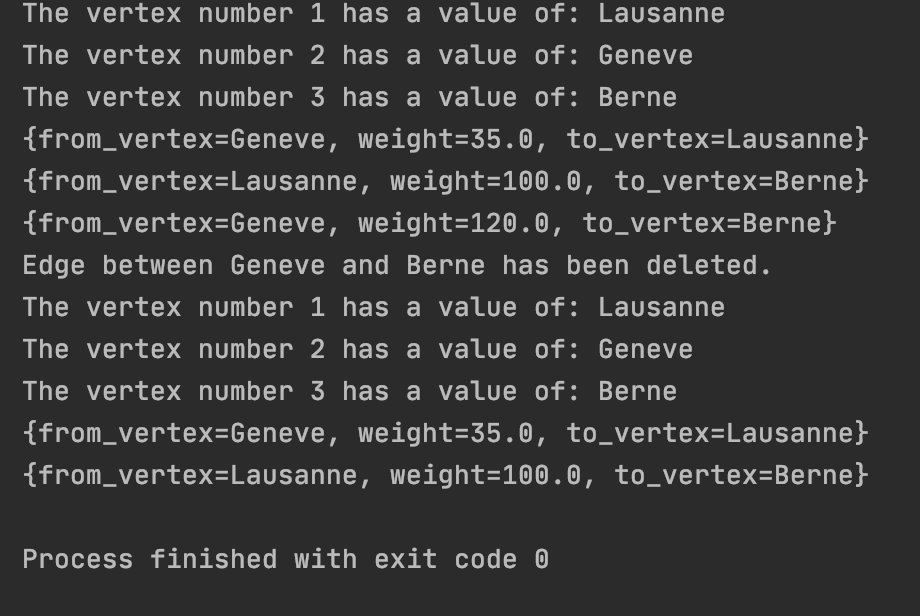
\includegraphics[]{ressources/sortie_juste.PNG}

\begin{Exercice}[20 minutes] Exercice 2\\

Voici une partie de la classe graph codée. Implémentez les méthodes "update\_weight", "new\_edge" et " "edge\_exist".
% TODO: Les guillemets contenus dans les commentaires du code cassent la coloration syntaxique. On devrait songer à les enlever.

\textbf{Java :}
         \lstinputlisting{ressources/graph_empty.java}
    \begin{enumerate}
        % TODO: les noms de méthodes doivent être identiques à celles du code.
        \item La méthode "update\_weight" doit prendre en paramètres: le sommet d'origine, le sommet d'arrivée ainsi que le poids d'une arête. Si cette arête existe alors elle change son poids. Sinon, elle imprimera une phrase indiquant que cette arête n'existe pas.
        \item La méthode "edge\_exist" qui va prendre en paramètre le sommet d'origine et le sommet d'arrivée. Si cette arête est dans le graph alors la méthode ressort son poids, 0 sinon.
        \item La méthode "new\_edge" doit créer une instance de Edges et l'ajouter à l'ensemble edges si la connexion n'existe pas déjà. Si elle existe avec un autre poids mettre à jour le poids. Si elle existe de façon identique alors retournez la dans la console avec print. Enfin, si on est dans aucun des deux cas précédents utiliser la méthode "generate\_edge" qui vous est donnée pour créer et ajouter cette arête au graph. La méthode "new\_edge" aura comme paramètres: le sommet d'origine, le sommet d'arrivée, le poids.
    \end{enumerate}

    \begin{conseil}
    \begin{enumerate}
    \item Utiliser une boucle for pour parcourir toutes les arêtes dans le graph. Faire un test sur les attributs de Edges pour changer le poids.
    \item Il faut tester pour chaque arête ( itération) si elle  est égale à celle rentrée en paramètres.
    \item Il faut utiliser les méthodes " edge\_exist", " update\_edge" et " generate\_edge" pour écrire cette méthode. Il y a 4 tests à effectuer: 
        \begin{enumerate}
        \item Si l'arête existe.
        \item Si l'arête existante a le même poids que celui indiqué en paramètre de la méthode.
        \item Si l'arête existante n'a pas le même poids que celui indiqué en paramètre de la méthode.
        \item Utilisez le résultat de " edge\_exist" pour simplifier ces tests.
        \end{enumerate}
    \end{enumerate}
    \end{conseil}
    \begin{solution}
    \textbf{Java :}
         \lstinputlisting{ressources/Edges.java}
    \end{solution}
    \begin{solution}
    \textbf{Java :}
         \lstinputlisting{ressources/graph.java}
    \end{solution}
    % TODO: Découper les fichiers de solutions pour qu'ils tiennent sur une page. Les renommer graph_1.java, graph_2,java par exemple et les mettre dans un dossier "Display" ou "Affichage". Mettre le fichier complet dans le dossier solution.
    \begin{solution}
    \textbf{Java :}
         \lstinputlisting{ressources/graph2.java}
    \end{solution}

\end{Exercice}


% TODO: Faire un exercice sur la POO en Python. On pourrait faire un truc simple (classe Point par exemple)
\section{Notions de POO en Python}
Dans cette section, nous créerons pas-à-pas une classe \lstinline{Point} contenant des attributs et des méthodes utiles.
Dans votre IDE, créez un nouveau projet Python (Fichier > Nouveau > Projet). Dans un dossier de votre choix, créez un fichier \lstinline{question} %TODO: Numéro de question à définir.

\begin{Exercice}[20 minutes]
    \begin{itemize}
        \item Créez une classe \lstinline{Point} et un constructeur à deux paramètres.
        \item Définissez deux attributs privés pour votre classe \lstinline{Point}. Ces attributs seront les coordonnées x et y de vos points.
        \item Définir des getters et setters.
        \item Définissez une méthode \lstinline{distance} qui prend en entrée self et p. \lstinline{self} représentant l'instance du point et \lstinline{p} représentant un autre point. Votre méthode \lstinline{distance} retournera la distance euclidienne entre le point \lstinline{self} et \lstinline{p}. Pour rappel, la distance euclidienne entre deux points est définie par la formule %TODO: Ecrire la formule de la distance entre deux points (Alpha).
        \item Définissez une méthode \lstinline{milieu} qui prendra en entrée \lstinline{self} et \lstinline{p} et qui retournera une instance d'un objet point situé entre \lstinline{self} et \lstinline{p}.
    \end{itemize}
    
    % TODO: Exercice à compléter (Alpha)
\end{Exercice}


\end{document}
